\documentclass[tikz,border=3pt]{standalone}
\usepackage{tikz}
\usetikzlibrary{positioning,shapes.geometric,shapes.misc,arrows.meta,fit,backgrounds,calc,decorations.pathmorphing,decorations.pathreplacing,shadows}
\usepackage[scaled]{helvet}
\renewcommand{\familydefault}{\sfdefault}
\definecolor{hon}{HTML}{1F6FB2}
\definecolor{honl}{HTML}{DCEBF7}
\definecolor{mal}{HTML}{C0392B}
\definecolor{mall}{HTML}{F8DEDB}
\definecolor{qnt}{HTML}{6C3FA0}
\definecolor{qntl}{HTML}{ECE3F6}
\definecolor{mec}{HTML}{1E8449}
\definecolor{mecl}{HTML}{DFF2E6}
\definecolor{grey}{HTML}{5D6D7E}
\tikzset{
  zone/.style={draw=grey!70, rounded corners=4pt, fill=gray!4, inner sep=5pt},
  patient/.style={circle, draw=hon, fill=honl, minimum size=6.5mm, inner sep=0pt, font=\scriptsize\bfseries, text=hon},
  badpat/.style={circle, draw=mal, fill=mall, minimum size=6.5mm, inner sep=0pt, font=\scriptsize\bfseries, text=mal},
  hub/.style={rectangle, rounded corners=1.5pt, draw=hon, fill=white, minimum width=5mm, minimum height=3.2mm, font=\tiny},
  peer/.style={rectangle, rounded corners=1.5pt, draw=hon, fill=honl, minimum width=9mm, minimum height=4.5mm, font=\tiny, align=center},
  box/.style={rectangle, rounded corners=3pt, draw, thick, align=center, font=\scriptsize, inner sep=3pt},
  lnk/.style={-{Stealth[length=1.6mm]}, thick, hon},
  d2d/.style={{Stealth[length=1.4mm]}-{Stealth[length=1.4mm]}, hon, dashed},
  atk/.style={-{Stealth[length=1.6mm]}, thick, mal, decorate, decoration={snake, amplitude=0.6mm, segment length=2.2mm, post length=1.5mm}},
  qlink/.style={qnt, line width=1.6pt, double=qntl, double distance=0.8pt},
  lab/.style={font=\tiny, align=center},
}
\begin{document}
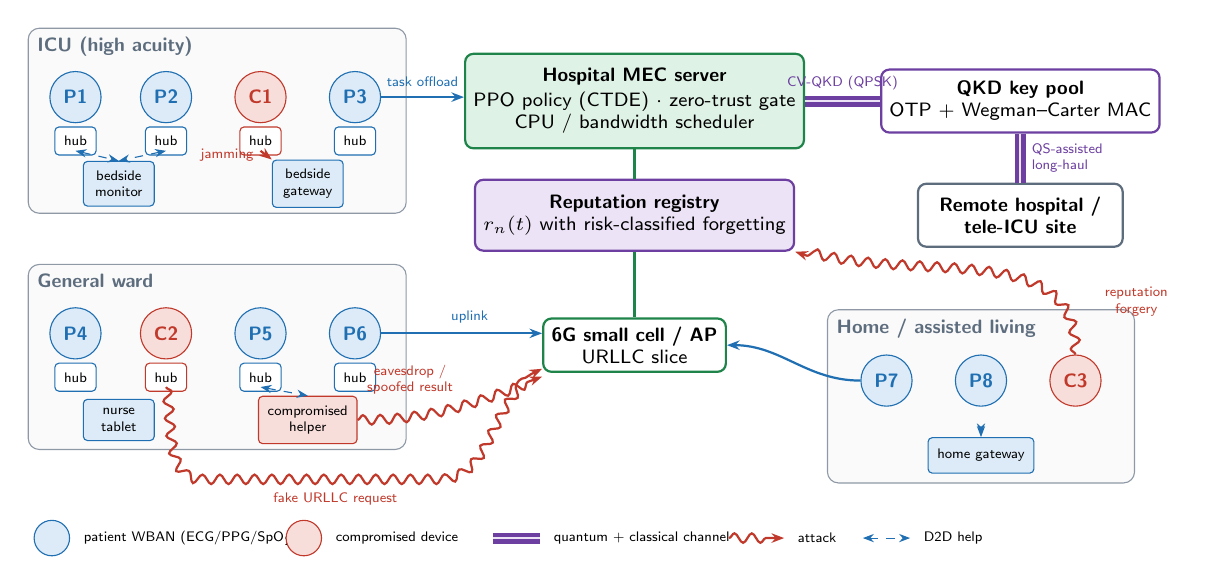
\begin{tikzpicture}[x=1cm,y=1cm]

% ---------------- hospital core (MEC + trust registry)
\node[box, draw=mec, fill=mecl, minimum width=3.5cm, minimum height=1.2cm] (mec) at (7.7,4.3)
 {\textbf{Hospital MEC server}\\[1pt] PPO policy (CTDE) $\cdot$ zero-trust gate\\ CPU / bandwidth scheduler};
\node[box, draw=qnt, fill=qntl, minimum width=3.5cm, minimum height=0.9cm] (reg) at (7.7,2.85)
 {\textbf{Reputation registry}\\ $r_n(t)$ with risk-classified forgetting};
\node[box, draw=mec, fill=white, minimum width=2.2cm] (ap) at (7.7,1.2) {\textbf{6G small cell / AP}\\ URLLC slice};
\draw[thick, mec] (mec.south) -- (reg.north);
\draw[thick, mec] (ap.north) -- (reg.south);
\node[box, draw=qnt, fill=white, minimum width=2.6cm, minimum height=0.8cm] (kp) at (12.6,4.3)
 {\textbf{QKD key pool}\\ OTP + Wegman--Carter MAC};
\node[box, draw=grey, fill=white, minimum width=2.6cm, minimum height=0.8cm] (rhosp) at (12.6,2.85)
 {\textbf{Remote hospital /}\\ \textbf{tele-ICU site}};
\draw[qlink] (mec.east) -- node[above, lab, text=qnt]{CV-QKD (QPSK)} (kp.west);
\draw[qlink] (kp.south) -- node[right, lab, text=qnt, align=left]{QS-assisted\\long-haul} (rhosp.north);

% ---------------- wards
\begin{scope}[on background layer]
\node[zone, minimum width=4.8cm, minimum height=2.35cm] (icu) at (2.4,4.05) {};
\node[zone, minimum width=4.8cm, minimum height=2.35cm] (ward) at (2.4,1.05) {};
\node[zone, minimum width=3.9cm, minimum height=2.2cm] (home) at (12.1,0.55) {};
\end{scope}
\node[font=\scriptsize\bfseries, text=grey, anchor=north west] at (icu.north west) {ICU (high acuity)};
\node[font=\scriptsize\bfseries, text=grey, anchor=north west] at (ward.north west) {General ward};
\node[font=\scriptsize\bfseries, text=grey, anchor=north west] at (home.north west) {Home / assisted living};

% patients ICU
\node[patient] (p1) at (0.6,4.35) {P1};
\node[patient] (p2) at (1.75,4.35) {P2};
\node[badpat]  (m1) at (2.95,4.35) {C1};
\node[patient] (p3) at (4.15,4.35) {P3};
\node[peer] (b1) at (1.15,3.25) {bedside\\monitor};
\node[peer] (b2) at (3.55,3.25) {bedside\\gateway};
\foreach \p in {p1,p2,p3} {\node[hub, below=0.4mm of \p] {hub};}
\node[hub, draw=mal, below=0.4mm of m1] {hub};

% patients ward
\node[patient] (p4) at (0.6,1.35) {P4};
\node[badpat]  (m2) at (1.75,1.35) {C2};
\node[patient] (p5) at (2.95,1.35) {P5};
\node[patient] (p6) at (4.15,1.35) {P6};
\node[peer] (b3) at (1.15,0.25) {nurse\\tablet};
\node[peer, draw=mal, fill=mall] (b4) at (3.55,0.25) {compromised\\helper};
\foreach \p in {p4,p5,p6} {\node[hub, below=0.4mm of \p] {hub};}
\node[hub, draw=mal, below=0.4mm of m2] {hub};

% home cell
\node[patient] (p7) at (10.9,0.75) {P7};
\node[patient] (p8) at (12.1,0.75) {P8};
\node[badpat] (m3) at (13.3,0.75) {C3};
\node[peer] (b5) at (12.1,-0.2) {home gateway};

% legitimate links
\draw[lnk] (p3.east) -- node[pos=0.5, above, lab]{task offload} (mec.west |- p3.east);
\draw[lnk] (p6.east) -- node[pos=0.55, above, lab]{uplink} (ap.west |- p6.east);
\draw[lnk] (p7.west) to[out=180,in=0] (ap.east);
\draw[d2d] (p1.south) ++(0,-0.35) -- (b1.north);
\draw[d2d] (p2.south) ++(0,-0.35) -- (b1.north);
\draw[d2d] (p5.south) ++(0,-0.35) -- (b4.north);
\draw[d2d] (p8.south) ++(0,-0.35) -- (b5.north);

% attacks
\draw[atk] (m1.south) ++(0,-0.35) -- node[left=0.3mm, lab, text=mal]{jamming} (b2.north west);
\draw[atk] (m2.south) ++(0,-0.35) to[out=-80,in=180] (2.2,-0.45) -- (5.2,-0.45) to[out=0,in=200] ([yshift=-3mm]ap.west);
\node[lab, text=mal, anchor=north] at (3.9,-0.55) {fake URLLC request};
\draw[atk] (b4.east) to[out=0,in=200] ([yshift=-4mm]ap.west);
\node[lab, text=mal, anchor=south] at (4.85,0.45) {eavesdrop /\\spoofed result};
\draw[atk] (m3.north) to[out=90,in=-20] (reg.south east);
\node[lab, text=mal, anchor=west] at (13.55,1.75) {reputation\\forgery};

% legend
\begin{scope}[shift={(0.3,-1.25)}]
\node[patient, minimum size=4.5mm] (l1) at (0,0) {};
\node[right=0.5mm of l1, font=\tiny] {patient WBAN (ECG/PPG/SpO$_2$)};
\node[badpat, minimum size=4.5mm] (l2) at (3.2,0) {};
\node[right=0.5mm of l2, font=\tiny] {compromised device};
\draw[qlink] (5.6,0) -- (6.2,0); \node[font=\tiny, anchor=west] at (6.25,0) {quantum + classical channel};
\draw[atk] (8.6,0) -- (9.3,0); \node[font=\tiny, anchor=west] at (9.35,0) {attack};
\draw[d2d] (10.3,0) -- (10.9,0); \node[font=\tiny, anchor=west] at (10.95,0) {D2D help};
\end{scope}
\end{tikzpicture}
\end{document}
